\section{Reverberation}
\gls{reverb} is an effect where the sound wave is reflected, and therefore the reflected waves haves another travelling time to the receiver than the initial sound directly from the source. This effect is a very frequently effect which happens each time sound can be reflected by walls, trees, table etc. The following \autoref{fig:reverb_reflect} shows the \gls{reverb} effect form one person to another person \citep{reverb_expl}.

\begin{figure} [htbp]
 \centering
  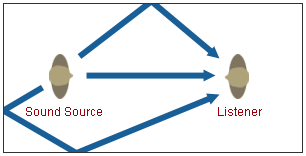
\includegraphics[width=0.7\textwidth]{reverb_reflect}
  \caption{The photo shows a echo in time domain}
  \label{fig:reverb_reflect}
\end{figure}

The received reflected sound is actually er series of very fast echo, which is maged together with all other reflected- and the direct sound, so the effect is notice the effect as one single effect, although that may be more than 100 echos. 

